\documentclass[14pt]{extbook}
\usepackage{multicol, enumerate, enumitem, hyperref, color, soul, setspace, parskip, fancyhdr} %General Packages
\usepackage{amssymb, amsthm, amsmath, bbm, latexsym, units, mathtools} %Math Packages
\everymath{\displaystyle} %All math in Display Style
% Packages with additional options
\usepackage[headsep=0.5cm,headheight=12pt, left=1 in,right= 1 in,top= 1 in,bottom= 1 in]{geometry}
\usepackage[usenames,dvipsnames]{xcolor}
\usepackage{dashrule}  % Package to use the command below to create lines between items
\newcommand{\litem}[1]{\item#1\hspace*{-1cm}\rule{\textwidth}{0.4pt}}
\pagestyle{fancy}
\lhead{Progress Quiz 4}
\chead{}
\rhead{Version A}
\lfoot{8448-1521}
\cfoot{}
\rfoot{Fall 2020}
\begin{document}

\begin{enumerate}
\litem{
Write the equation of the graph presented below in the form $f(x)=ax^2+bx+c$, assuming  $a=1$ or $a=-1$. Then, choose the intervals that $a, b,$ and $c$ belong to.
\begin{center}
    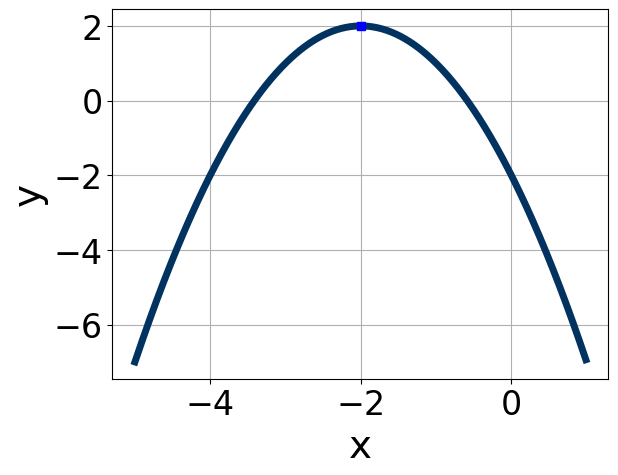
\includegraphics[width=0.5\textwidth]{../Figures/quadraticGraphToEquationCopyA.png}
\end{center}
\begin{enumerate}[label=\Alph*.]
\item \( a \in [-2.4, -0.7], \hspace*{5mm} b \in [-5, -2], \text{ and } \hspace*{5mm} c \in [-2, 2] \)
\item \( a \in [-2.4, -0.7], \hspace*{5mm} b \in [0, 6], \text{ and } \hspace*{5mm} c \in [-2, 2] \)
\item \( a \in [0.3, 2], \hspace*{5mm} b \in [0, 6], \text{ and } \hspace*{5mm} c \in [6, 8] \)
\item \( a \in [0.3, 2], \hspace*{5mm} b \in [-5, -2], \text{ and } \hspace*{5mm} c \in [6, 8] \)
\item \( a \in [-2.4, -0.7], \hspace*{5mm} b \in [0, 6], \text{ and } \hspace*{5mm} c \in [-8, -5] \)

\end{enumerate} }
\litem{
Factor the quadratic below. Then, choose the intervals that contain the constants in the form $(ax+b)(cx+d); b \leq d.$\[ 24x^{2} -2 x -15 \]\begin{enumerate}[label=\Alph*.]
\item \( a \in [16.3, 19.4], \hspace*{5mm} b \in [-8, -3], \hspace*{5mm} c \in [0, 2], \text{ and } \hspace*{5mm} d \in [2, 9] \)
\item \( a \in [2.8, 3.5], \hspace*{5mm} b \in [-8, -3], \hspace*{5mm} c \in [6, 10], \text{ and } \hspace*{5mm} d \in [2, 9] \)
\item \( a \in [-2.2, 1.3], \hspace*{5mm} b \in [-21, -19], \hspace*{5mm} c \in [0, 2], \text{ and } \hspace*{5mm} d \in [11, 21] \)
\item \( a \in [5.4, 9.7], \hspace*{5mm} b \in [-8, -3], \hspace*{5mm} c \in [2, 6], \text{ and } \hspace*{5mm} d \in [2, 9] \)
\item \( \text{None of the above.} \)

\end{enumerate} }
\litem{
Solve the quadratic equation below. Then, choose the intervals that the solutions belong to, with $x_1 \leq x_2$ (if they exist).\[ 14x^{2} +10 x -7 = 0 \]\begin{enumerate}[label=\Alph*.]
\item \( x_1 \in [-18.2, -14.7] \text{ and } x_2 \in [5.64, 6.2] \)
\item \( x_1 \in [-0.8, -0.1] \text{ and } x_2 \in [0.96, 2.01] \)
\item \( x_1 \in [-2.1, -0.8] \text{ and } x_2 \in [-0.2, 0.87] \)
\item \( x_1 \in [-24, -22.3] \text{ and } x_2 \in [21.55, 22.01] \)
\item \( \text{There are no Real solutions.} \)

\end{enumerate} }
\litem{
Solve the quadratic equation below. Then, choose the intervals that the solutions $x_1$ and $x_2$ belong to, with $x_1 \leq x_2$.\[ 10x^{2} -53 x + 36 = 0 \]\begin{enumerate}[label=\Alph*.]
\item \( x_1 \in [0.86, 0.91] \text{ and } x_2 \in [3.17, 4.26] \)
\item \( x_1 \in [0.19, 0.32] \text{ and } x_2 \in [13.5, 13.94] \)
\item \( x_1 \in [7.99, 8.09] \text{ and } x_2 \in [44.48, 45.43] \)
\item \( x_1 \in [1.54, 1.67] \text{ and } x_2 \in [2.08, 2.32] \)
\item \( x_1 \in [0.7, 0.83] \text{ and } x_2 \in [4.42, 4.87] \)

\end{enumerate} }
\litem{
Solve the quadratic equation below. Then, choose the intervals that the solutions belong to, with $x_1 \leq x_2$ (if they exist).\[ 16x^{2} +13 x -2 = 0 \]\begin{enumerate}[label=\Alph*.]
\item \( x_1 \in [-16.56, -15] \text{ and } x_2 \in [1.7, 4.2] \)
\item \( x_1 \in [-0.62, 0.47] \text{ and } x_2 \in [0.6, 2.1] \)
\item \( x_1 \in [-18.41, -17.46] \text{ and } x_2 \in [15.1, 17.6] \)
\item \( x_1 \in [-1.29, -0.67] \text{ and } x_2 \in [-0.3, 0.5] \)
\item \( \text{There are no Real solutions.} \)

\end{enumerate} }
\litem{
Graph the equation below.\[ f(x) = -(x+1)^2 - 13 \]\begin{enumerate}[label=\Alph*.]
\begin{multicols}{2}\item 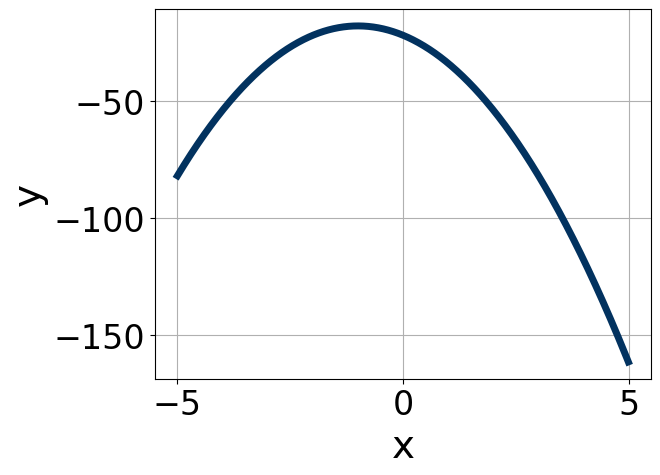
\includegraphics[width = 0.3\textwidth]{../Figures/quadraticEquationToGraphAA.png}\item 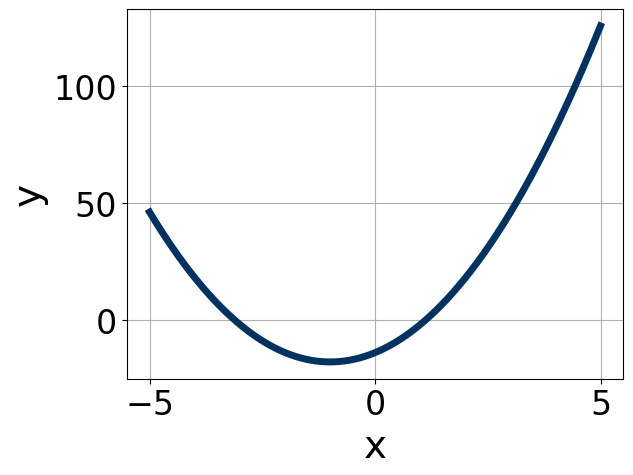
\includegraphics[width = 0.3\textwidth]{../Figures/quadraticEquationToGraphBA.png}\item 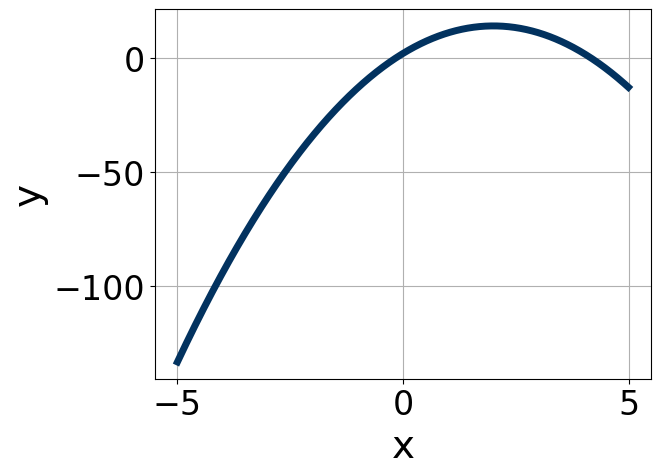
\includegraphics[width = 0.3\textwidth]{../Figures/quadraticEquationToGraphCA.png}\item 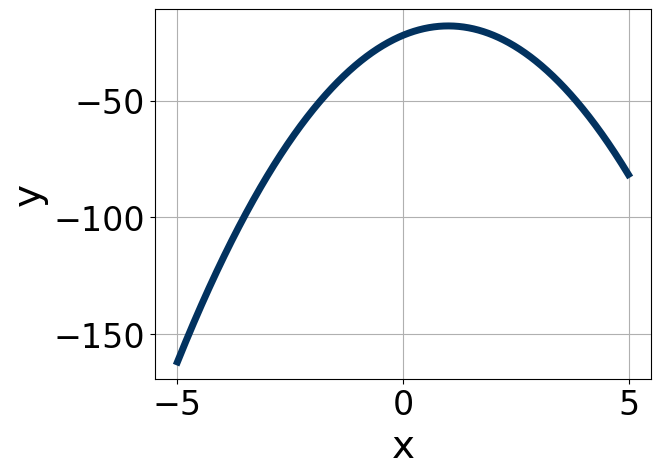
\includegraphics[width = 0.3\textwidth]{../Figures/quadraticEquationToGraphDA.png}\end{multicols}\item None of the above.
\end{enumerate} }
\litem{
Factor the quadratic below. Then, choose the intervals that contain the constants in the form $(ax+b)(cx+d); b \leq d.$\[ 36x^{2} -25 x -25 \]\begin{enumerate}[label=\Alph*.]
\item \( a \in [7.4, 10], \hspace*{5mm} b \in [-8, 1], \hspace*{5mm} c \in [3.4, 5.1], \text{ and } \hspace*{5mm} d \in [5, 7] \)
\item \( a \in [3.1, 6], \hspace*{5mm} b \in [-8, 1], \hspace*{5mm} c \in [7.8, 9.2], \text{ and } \hspace*{5mm} d \in [5, 7] \)
\item \( a \in [-0.3, 3.2], \hspace*{5mm} b \in [-8, 1], \hspace*{5mm} c \in [24.6, 27.4], \text{ and } \hspace*{5mm} d \in [5, 7] \)
\item \( a \in [-0.3, 3.2], \hspace*{5mm} b \in [-45, -40], \hspace*{5mm} c \in [-1.8, 1.8], \text{ and } \hspace*{5mm} d \in [18, 23] \)
\item \( \text{None of the above.} \)

\end{enumerate} }
\litem{
Solve the quadratic equation below. Then, choose the intervals that the solutions $x_1$ and $x_2$ belong to, with $x_1 \leq x_2$.\[ 15x^{2} +2 x -24 = 0 \]\begin{enumerate}[label=\Alph*.]
\item \( x_1 \in [-1.93, -0.85] \text{ and } x_2 \in [1.06, 1.39] \)
\item \( x_1 \in [-5.12, -3.17] \text{ and } x_2 \in [-0.03, 0.57] \)
\item \( x_1 \in [-0.94, -0.1] \text{ and } x_2 \in [3.38, 3.79] \)
\item \( x_1 \in [-3.16, -1.49] \text{ and } x_2 \in [0.41, 1.16] \)
\item \( x_1 \in [-21.25, -18.48] \text{ and } x_2 \in [17.82, 18.2] \)

\end{enumerate} }
\litem{
Graph the equation below.\[ f(x) = -(x-2)^2 - 10 \]\begin{enumerate}[label=\Alph*.]
\begin{multicols}{2}\item 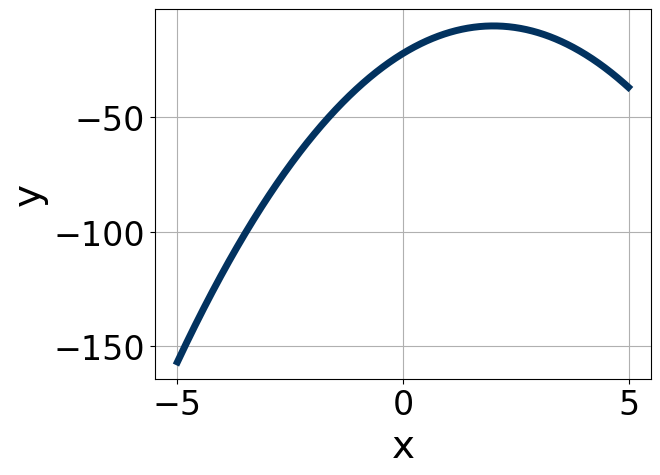
\includegraphics[width = 0.3\textwidth]{../Figures/quadraticEquationToGraphCopyAA.png}\item 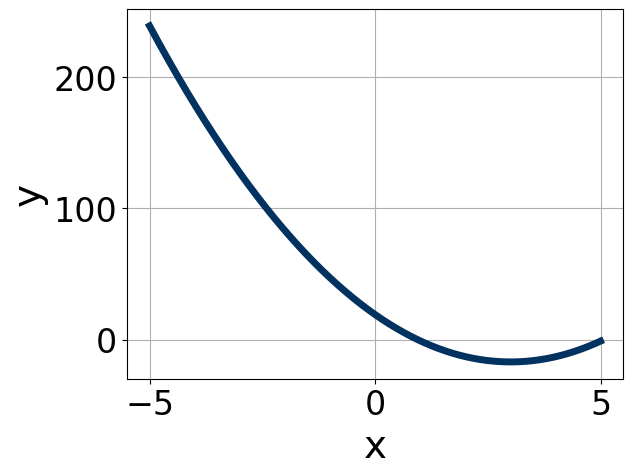
\includegraphics[width = 0.3\textwidth]{../Figures/quadraticEquationToGraphCopyBA.png}\item 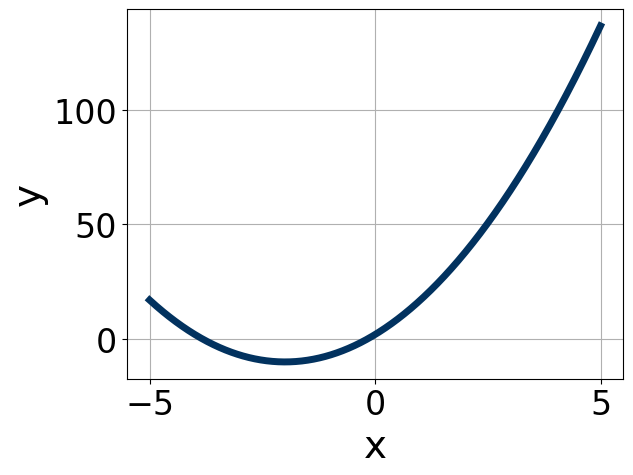
\includegraphics[width = 0.3\textwidth]{../Figures/quadraticEquationToGraphCopyCA.png}\item 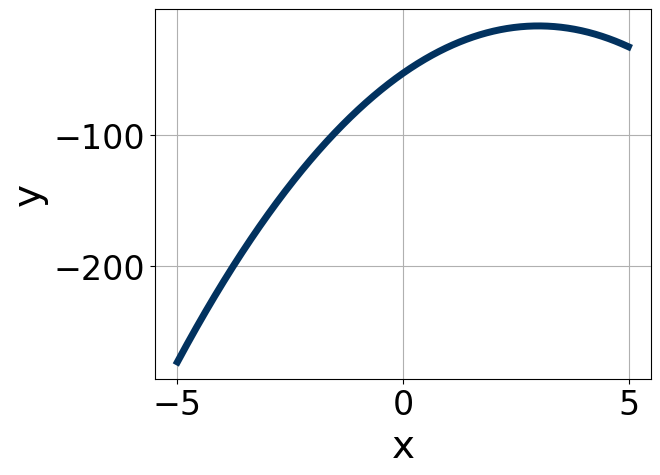
\includegraphics[width = 0.3\textwidth]{../Figures/quadraticEquationToGraphCopyDA.png}\end{multicols}\item None of the above.
\end{enumerate} }
\litem{
Write the equation of the graph presented below in the form $f(x)=ax^2+bx+c$, assuming  $a=1$ or $a=-1$. Then, choose the intervals that $a, b,$ and $c$ belong to.
\begin{center}
    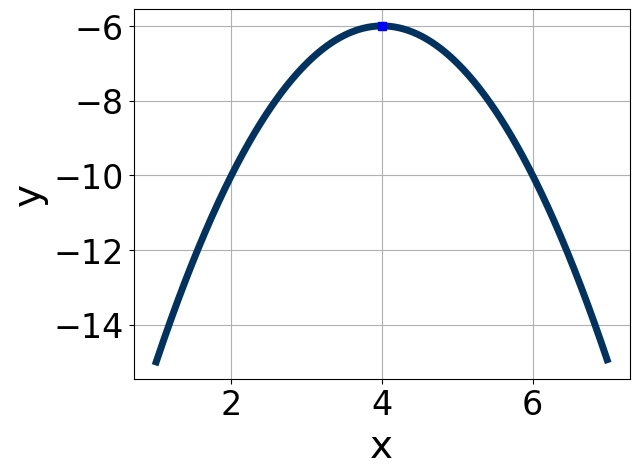
\includegraphics[width=0.5\textwidth]{../Figures/quadraticGraphToEquationA.png}
\end{center}
\begin{enumerate}[label=\Alph*.]
\item \( a \in [-1, 0], \hspace*{5mm} b \in [8, 10], \text{ and } \hspace*{5mm} c \in [-23, -19] \)
\item \( a \in [0, 5], \hspace*{5mm} b \in [-9, 0], \text{ and } \hspace*{5mm} c \in [7, 12] \)
\item \( a \in [-1, 0], \hspace*{5mm} b \in [-9, 0], \text{ and } \hspace*{5mm} c \in [-23, -19] \)
\item \( a \in [0, 5], \hspace*{5mm} b \in [8, 10], \text{ and } \hspace*{5mm} c \in [7, 12] \)
\item \( a \in [-1, 0], \hspace*{5mm} b \in [-9, 0], \text{ and } \hspace*{5mm} c \in [-12, -9] \)

\end{enumerate} }
\end{enumerate}

\end{document}